\PassOptionsToPackage{full}{textcomp}
\documentclass[]{tufte-handout}
%\usepackage{fontspec}

% load babel package and options here
%\usepackage[p,osf]{ETbb} % osf in text, tabular lining figures in math
\usepackage{ETbb} % osf in text, tabular lining figures in math
\usepackage[scaled=.95,type1]{cabin} % sans serif in style of Gill Sans
\usepackage[varqu,varl]{zi4}% inconsolata typewriter
\usepackage[T1]{fontenc} % LY1 also works
\usepackage[libertine,vvarbb]{newtxmath}
%\usepackage[cal=boondoxo,bb=boondox,frak=boondox]{mathalfa}

%\geometry{showframe} % display margins for debugging page layout

\usepackage{graphicx} % allow embedded images
%  \setkeys{Gin}{width=\linewidth,totalheight=\textheight,keepaspectratio}
  \graphicspath{{graphics/}} % set of paths to search for images
\usepackage{amsmath}  % extended mathematics
\usepackage{booktabs} % book-quality tables
%\usepackage{units}    % non-stacked fractions and better unit spacing
\usepackage{multicol} % multiple column layout facilities
\usepackage{lipsum}   % filler text
\usepackage{fancyvrb} % extended verbatim environments
  \fvset{fontsize=\normalsize}% default font size for fancy-verbatim environments
\usepackage{gensymb} % provides symbols like \degree
\usepackage{ragged2e} % enables hyphenation in ragged-right justification
\usepackage[normalize-symbols]{textalpha} %enables \textalpha for alpha symbol etc.

\usepackage{hyperref} % enables styling of href and url
\hypersetup{
    pdftitle={Mechanisms},
    pdfauthor={Barry Linkletter},
    colorlinks=true,
    linkcolor=blue,
    filecolor=magenta,      
    urlcolor=blue,
    pdfborder={0 0 0},
    frenchlinks=false,
    pdfpagemode=FullScreen,
    }
    \urlstyle{same}
\makeatletter
% Inspired by http://anti.teamidiot.de/nei/2009/09/latex_url_slash_spacingkerning/
% but slightly less kern and shorter underscore
\let\UrlSpecialsOld\UrlSpecials
\def\UrlSpecials{\UrlSpecialsOld\do\/{\Url@slash}\do\_{\Url@underscore}}%
\def\Url@slash{\@ifnextchar/{\kern-.03em\mathchar47\kern-.15em}%
    {\kern-.0em\mathchar47\kern-.08em\penalty\UrlBigBreakPenalty}}
\def\Url@underscore{\nfss@text{\leavevmode \kern.06em\vbox{\hrule\@width.3em}}}
\makeatother

%\usepackage{enumitem} % allows resuming enumerate lists.
\usepackage{mathtools}
\usepackage{mhchem}

\usepackage{siunitx} % provides "S" column class for aligning decimals.  
         \sisetup{uncertainty-mode = separate}

\usepackage{nicefrac}

\usepackage[nospace]{varioref}
    \renewcommand\reftextfaceafter{on the following page}
    \renewcommand\reftextafter {on the next page}
    \renewcommand\reftextfacebefore{on the previous page}
    \renewcommand\reftextbefore {on the previous page}

\newcommand{\tss}[1]{\textsuperscript{#1}}

\usepackage[english]{babel}
\usepackage{float}
\usepackage{stackrel}

\usepackage[shortconst]{physconst}

\usepackage[normalem]{ulem}  % provides strikethrough \sout{}

\usepackage{newfloat}
\DeclareFloatingEnvironment[
  fileext = los ,
  listname = {List of Schemes} ,
  name = Scheme
]{scheme}

\usepackage{newfloat}
\DeclareFloatingEnvironment[
  fileext = loe ,
  listname = {List of Eqs} ,
  name = Equation
]{equate}

\usepackage{listings}
\usepackage{longtable}

%%%%%%%%%%%%%%%%%%%%%%%%%%%%%%%%%%%%%%%%%%%%%%%%%%%%%%%%%%%
% Plot Symbols
\usepackage{tikz}
\newcommand*{\priority}[1]{\begin{tikzpicture}[scale=0.085]%
    \draw[thick] (0,0) circle (1);
    \fill[fill opacity=1,fill=black] (0,0) -- (90:{#1>0?1:0}) arc (90:90-#1*3.6:1) -- cycle;
    \end{tikzpicture}}

%\let\Bbbk\relax
%\usepackage{amssymb}

%%%%%%%%%%%%%%%%%%%%%%%%%%%%%%%%%%%%%%%%%%%%%%%%%%%%%%%%%%%

\title{A Hunt for Data}
\author[Barry Linkletter]{Barry Linkletter}
\date{} % without \date command, current date is supplied


\begin{document}

\justifying

\maketitle
\marginnote[-15mm]{This document was produced using the \LaTeX\ typesetting language with the Tufte-handout document class. Chemical diagrams were created in \textit{ChemDoodle} and calculations and plotting were performed using \textit{Python} tools in a \textit{Jupyter Notebook}. Diagrams and plots were further edited in \textit{Affinity Designer}\vspace{3mm}}
%\justify
\begin{abstract}

\noindent In our exploration of the mechanism of ester hydrolysis in extreme acid condition we have examined the work of Yates and the example of methyl acetate hydrolysis.\sidenote[][-0mm]
{``Mechanisms of ester hydrolysis in aqueous sulfuric acids.''
K. Yates, R.A. McClelland,
\textit{J. Am. Chem. Soc.}, \textbf{1967}, \textit{89}, 2686-2692.
\url{https://doi.org/10.1021/ja00987a033} \label{ref:ref1}}
That work presents plots of data for ethyl acetate hydrolysis but does not provide the data. the authors refers to other papers for the source. In addition there is a plot of methyl acetate hydrolysis showing points that are from more concentrated acid conditions than are presented in the data tables. We will get that data and document the process with this report and a \textit{Python} notebook.

\end{abstract}




\section{More Extreme Conditions for Methyl Acetate}

In Figure~1 of the Yates paper\tss{\ref{ref:ref1}} we see three points at the most extreme acidities that are not included in the data presented in Table~1 of that paper. I believe that this was an error due to Yates and McClelland performing all their calculations in the interpretation of the methyl acetate data using only the rates that represent the $AAc2$ mechanism. The final three points (and as we concluded, the fourth-last point as well) contain significant or predominant contributions from the $AAc1$ mechanism and so were not used. Then when it was time to make the paper they printed the data that they were using, not all the data that they had collected. We will need to perform some data archeology to get these values.

\begin{marginfigure}[0mm]
  \centering
  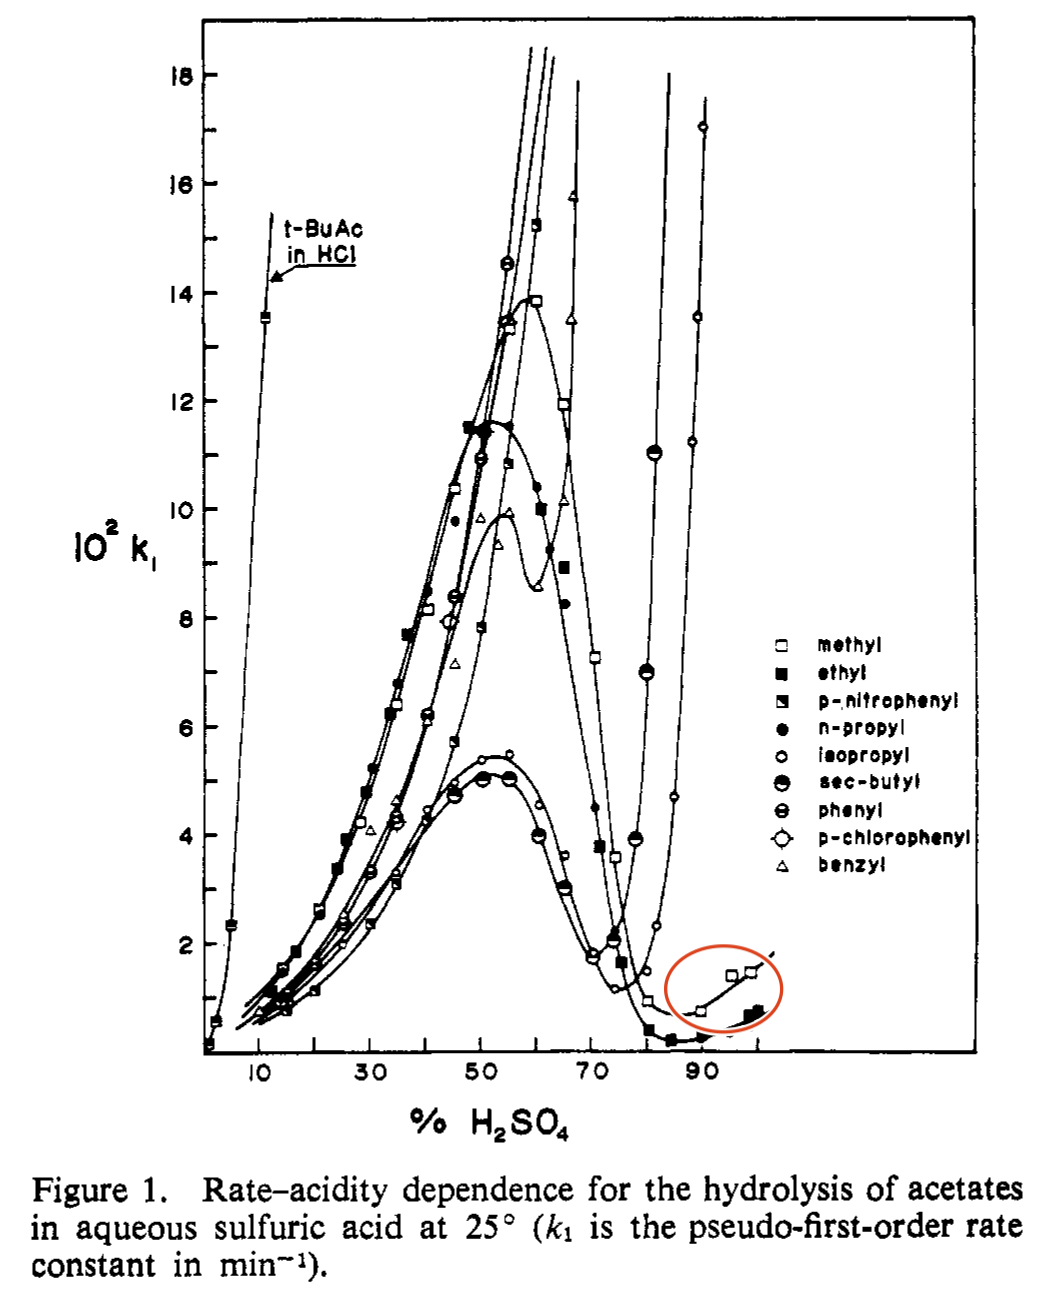
\includegraphics[width=150pt]{images/Yates-McClelland-1967-F1.png}
  \caption[0mm]{Plot of the observed pseudo first-order rate constants, $k_{obs}$, for ester hydrolysis in aqueous sulfuric acid presented as Figure~1 in Yates, 1967.\tss{\ref{ref:ref1}}  $\uparrow$ \\ The open squares that are circled in the lower right corner are not included in the data table of Yates, 1967.\tss{\ref{ref:ref1}}  \vspace{3mm}}
  \label{fig:fig1}
\end{marginfigure}

\subsection{Extracting Data from the Plot}
I will use a plot digitizer app\sidenote[][0mm]{WebPlotDigitizer from \url{https://automeris.io}. Accessed Sept. 26, 2025. Use the archived version 4 that you can download and run on your own computer. The current version 5 is now a website for which you need to create an account, surrender personal information and endure ``AI assistance.''} to convert the graphic points to data points. I will capture as many points as I can for the methyl acetate data (some are obscured in the image by other points) and compare the digitized data to the reported data to confirm the accuracy of the picked points.

The data points from Table~1 of the Yates paper and the digitized points are shown in Table~\vref{tab:tab1} of this document. The reported data and the digitized data were plotted together and are presented in Figure~\ref{fig:fig2}. Where data exists from both sources, strong agreement was observed. There seemed to be a general slight shift to the right for most data points and one point seemed to show a significant difference. The differentials are plotted in Figure~\ref{fig:fig3} and show the outlier clearly. Ignoring the outlier we observe that the digitization accurately identified the values for $k_{obs}$ (mean differential of $0.00 \pm 0.02$, ignoring the outlier) but there was a significant deviation in values for \%\ce{H2SO4} (mean differential of $0.37 \pm 0.14$).



\begin{table}[h!]
\caption[][0mm]{Reported data for methyl acetate hydrolysis compared with data extracted from a plot in Yates, 1967.\tss{\ref{ref:ref1}}\\ $\longleftarrow$\\ Bold data points were extracted from the plot image but are absent in the reported values in the paper. One point in the plot was not able to be identified due to the quality of the image.\\ \vspace{10mm} The \textit{Python} notebooks that describe Figures~\ref{fig:fig2} and \ref{fig:fig3} on this page can accessed via Google Colab at \url{https://colab.research.google.com/github/blinkletter/4410PythonNotebooks/blob/main/Class_30_Yates_New/Yates-MeOAc-Data.ipynb}}

\centering
    \begin{tabular}{SSSS}
%        \toprule
        {\%\ce{H2SO4} } & {$k_{obs}$}     & {\%\ce{H2SO4} } & {$k_{obs}$}  \\
        \midrule
14.1 &          1.50       &  14.48  &     1.52     \\
20.7 &          2.61       &  20.98  &     2.65     \\
28.3 &          4.22       &  28.49  &     4.23     \\
34.8 &          6.41       &  35.01  &     6.40     \\
40.4 &          8.14       &  40.91  &     8.15     \\
45.4 &         10.4        &  45.82  &     10.37    \\
50.2 &         11.4        &           &              \\
55.2 &         13.3        &  55.79   &     13.30   \\
60.4 &         13.8        &  60.65   &     13.81   \\
65.2 &         11.9        &  65.45   &     11.92   \\
70.4 &          7.25       &  70.99   &     7.25    \\
74.1 &          3.83       &  74.53   &     3.57    \\
80.0 &          0.931      &  80.33   &     0.91    \\
      &                    &    \textbf{90.02}   &     \textbf{0.72}    \\ 
      &                    &    \textbf{95.69}   &     \textbf{1.38}     \\
      &                    &    \textbf{99.13}   &     \textbf{1.44}     \\
%        \bottomrule
    \end{tabular} \label{tab:tab1}
\end{table}


\begin{figure}[h!]
\vspace{15mm}
  \centering
  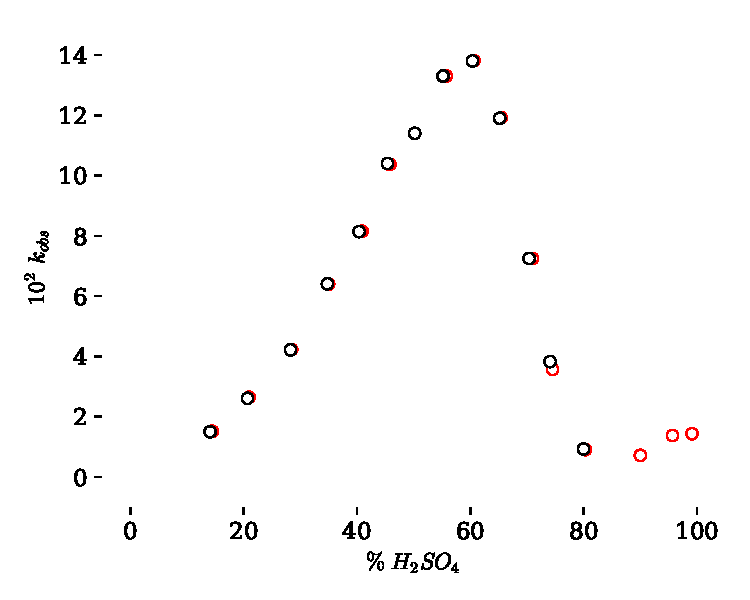
\includegraphics[scale=0.7]{images/plot1}
  \caption[][15mm]{Plot of data reported in Table~1 (black circles) and data digitized from Figure~1 (red circles) from Yates, 1967 for methyl acetate hydrolysis.\tss{\ref{ref:ref1}}   \\  $\longleftarrow$ \vspace{3mm}}
  \label{fig:fig2}
\end{figure}

\begin{marginfigure}[-60mm]
  \centering
  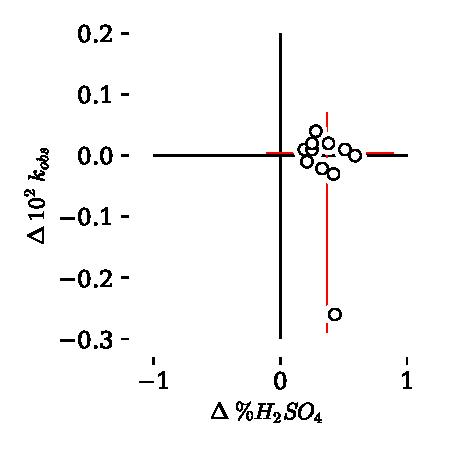
\includegraphics[width=150pt]{images/plot2}
  \caption[0mm]{Plot of the differentials for reported and digitized data for methyl acetate hydrolysis in Yates, 1967.\tss{\ref{ref:ref1}} $\uparrow$ \\ The median differentials for each parameter as shown on the plot in red. the outlier was ignored for calculating mean values. The median deflection on the x-axis was 0.37. The data digitized from the three missing points was adjusted accordingly when compiled in Table~\vref{tab:all1}.\vspace{3mm}}
  \label{fig:fig3}
\end{marginfigure}

\subsection{Correcting the Data Set}

Given the mean differential for the \%\ce{H2SO4} it was decided to correct the digitized data by the value of 0.37. This brought the value of \%\ce{H2SO4} to the same values as used for the data series for isopropyl acetate. This increases my confidence that I made the right choice. The single large differential observed for the point at \qty{60}{\percent}  \ce{H2SO4} is more difficult to interpret. the difference between the reported value and the value in the plot is about $-0.26$. If the value reported in the table for $k_{obs}$ was 13.6 instead of 13.8 then we would be close to the digitized value. The numerals 6 and 8 are easily confused when converting data from the notebook to a typeset document. Could the lab have operated with a value of 13.6 is all their calculations but the typesetting erroneously switched it to 13.8? Does this theory justify using a value of 13.6 instead of the reported value? I will keep the reported value but stay aware of this discrepancy.

\section{The Data for Ethyl Acetate}

Yates and McClelland discuss results for ethyl acetate hydrolysis and include the values in the plots and data analysis. But they do not provide the data in table~1 of the paper.\tss{\ref{ref:ref1}} The reference older work and send the reader searching for that data.\sidenote[][-15mm]{``The Possibility of a Cyclic Mechanism for Acid-Catalyzed Ester Hydrolysis.'' C.A. Lane, M.F. Cheung, G.F. Dorsey, \textit{J. Am. Chem. Soc.}, \textbf{1968}, \textit{90}, 6492–6494. \url{https://doi.org/10.1021/ja01025a046}.\label{ref:lane} \vspace{2mm}}\tss{,}\sidenote[][0mm]{``The Kinetics of Ester Hydrolysis in Concentrated Aqueous Acids.'' R.P. Bell, A.L. Dowding, J.A. Noble,  \textit{J. Chem. Soc.}, \textbf{1955}, 3106–3110. \url{https://doi.org/10.1039/JR9550003106}\label{ref:bell}\vspace{2mm}}\tss{,}\sidenote{``The Hydrolysis of Ethyl Acetate in Concentrated Aqueous Sulphuric Acid.'' D. Jaques,  \textit{J. Chem. Soc.} \textbf{1965}, 3854–3904. \url{https://doi.org/10.1039/JR9650003854} \label{ref:jaques}. For a good introduction to the math used to interpret the data see ``Hydrolysis of Ethyl Acetate in Concentrated Sulfuric Acid. A Group Experiment for Advanced Students.'' D. Jaques, \textit{J. Chem. Educ.}, \textbf{1971}, \textit{48}, 623-625. \url{https://doi.org/10.1021/ed048p623}.\vspace{2mm}} So off I go.

\subsection{Lane et al., 1968\tss{\ref{ref:lane}}}

This data set presents literature data from Bell et al., 1955\tss{\ref{ref:bell}} along with more experimental data determined using the same methods as Bell. The data is presented in figure~\vref{fig:lanetable1}. Take note of the data presented for the activity of water, $a_{H_2O}$, the extent of protonation of the ester, $\nicefrac{[BH]}{[BH^+]}$, and the value of $k_{BH^+}$, which I presume is the first-order rate constant for hydrolysis of the protonated intermediate. The $k_{BH^+}$ term is not discussed in the paper so I don't know why it is presented. Also, in my initial reading of the data table I was unable to reproduce it from the data presented. I'll have to look into it another time.

\begin{figure}[h!]
\vspace{0mm}
  \centering
  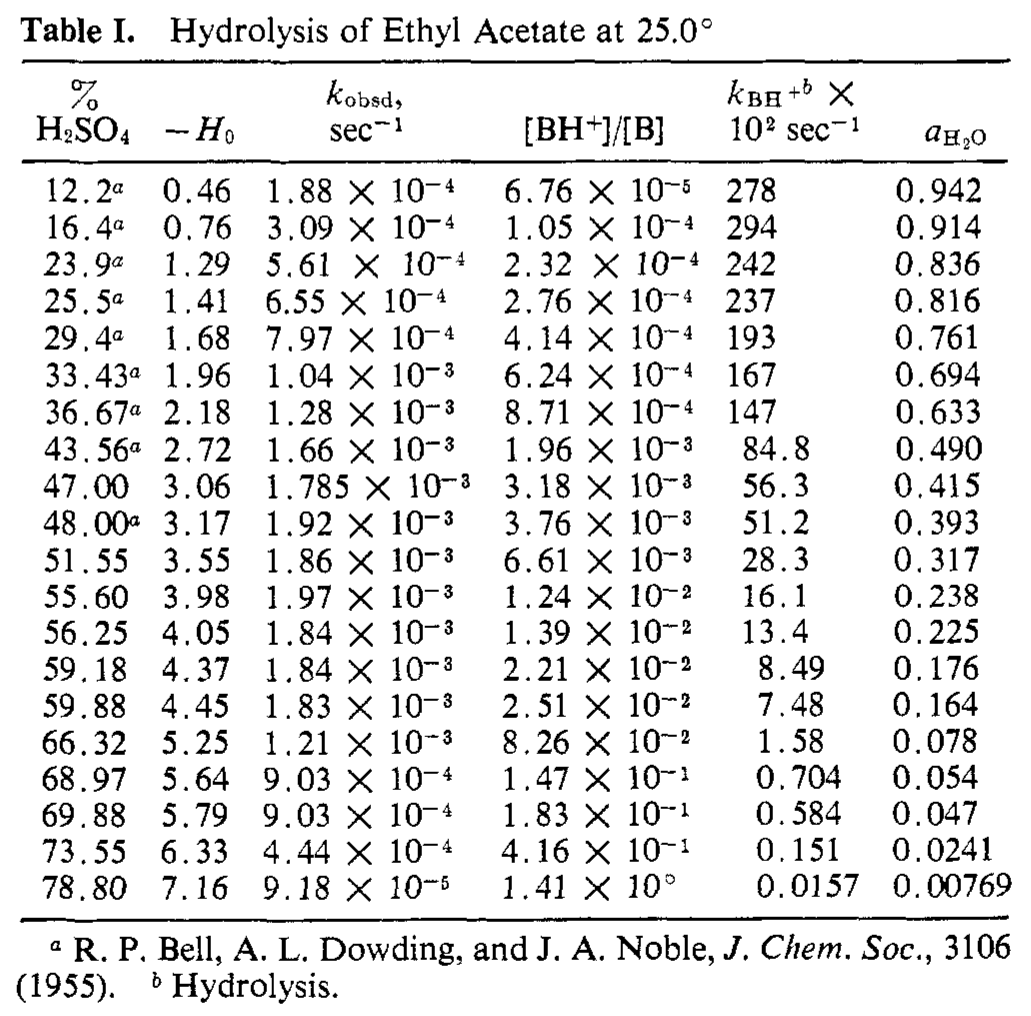
\includegraphics[scale=0.2]{images/LaneTable1}
  \caption[][5mm]{table~1 from Lane et al., 1968\tss{\ref{ref:lane}}   \\  $\longleftarrow$ \vspace{3mm}}
  \label{fig:lanetable1}
\end{figure}



\subsection{Bell et al., 1955\tss{\ref{ref:bell}}}

\begin{marginfigure}[0mm]
\vspace{0mm}
  \centering
  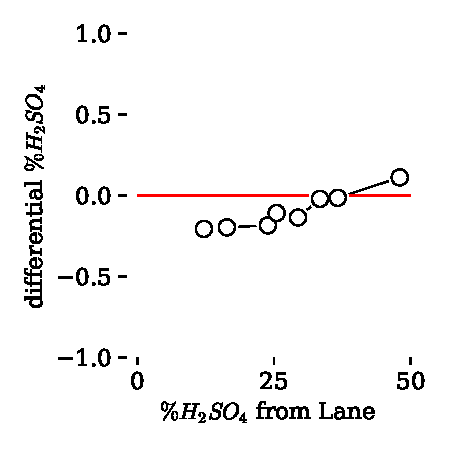
\includegraphics[scale=0.6]{images/plot4} \\
  \caption{Differential plot for the difference between the \% concentrations of \ce{H2SO4} calculated by Lane\tss{\ref{ref:lane}} from the molar concentrations reported by Bell\tss{\ref{ref:bell}}  and the same from my own interpolation of the modern tables in the 105\tss{th} edition of the CRC Handbook. $\uparrow$ \vspace{3mm}}

  \label{fig:belldatadiff}
\end{marginfigure}



You can see that about half of the data presented by Lane was from previous work by Bell et al., 1955\tss{\ref{ref:bell}}. The data from Bell is presented in Figure~\vref{fig:belldata}. You can see that it does not include any information about , $a_{H_2O}$, $\nicefrac{[BH]}{[BH^+]}$, or $k_{BH^+}$. These values would have been calculated by lane using the available data, some of which was likely communicated privately. Also note that the concentrations of sulphuric acid are reported in Molar, not \%\ce{H2SO4} and the $H_0$ values differ slightly. Lane would have converted molarity to \%\ce{H2SO4} and used more recent data for the $H_0$ values of sulphuric acid mixtures, specifically the values reported by Jorgenson in 1963 (see reference 8 in Lane\tss{\ref{ref:lane}}). Speaking of more modern values, I used the tables in the 105\tss{th} edition of the CRC handbook to convert Bell's molar concentration value to \% mass and obtained very similar values to those reported by Lane. Figure~\vref{fig:belldatadiff} presents a plot of these differences. You can see that the differences are small, but systematic. This reflects the small difference in the data tables between 1960 and 2025.


\begin{figure}[h!]
\vspace{0mm}
  \centering
  \includegraphics[scale=0.18]{images/Belltable1A.png} \\
  \includegraphics[scale=0.18]{images/Belltable1B.png}
  \caption[][0mm]{Table~1 from Bell et al., 1955\tss{\ref{ref:bell}}  \\  $\longleftarrow$ \vspace{3mm}}

  \label{fig:belldata}
\end{figure}


To convert moles/L to \%\ce{H2SO4} we will need a table of density data for various concentrations of sulphuric acid. The CRC Handbook presents a table that will convert molar concentration to density and \%\ce{H2SO4}. See the discussion presented in ``Interpolating Literature Data Sets'' on the Moodle site. The results of converting the molar concentrations to percent mass are presented in Table~\vref{tab:tab2}.
\begin{table}[h!]
\caption[][0mm]{Molar concentrations of \ce{H2SO4} from Bell\tss{\ref{ref:bell}} converted to \%\ce{H2SO4} and compared to the \%\ce{H2SO4} values reported by Lane\tss{\ref{ref:lane}} for the same data. The reported $H_0$ values used by Bell and Lane are also compared. See Figure~\vref{fig:belldatadiff} for a plot of the differentials between the two sets of interpolated  \%\ce{H2SO4} values. \\ $\longleftarrow$\\ \vspace{5mm} The \textit{Python} notebooks that describe how the data was interpolated can accessed via Google Colab at \url{https://colab.research.google.com/github/blinkletter/4410PythonNotebooks/blob/main/Class_30_Yates_New/Bell-EtOAc-Data.ipynb}}

\centering
    \begin{tabular}{SSSSS}
%        \toprule
\multicolumn{2}{c}{Data reported by Bell} & {Interpolated} & \multicolumn{2}{c}{Data reported by Lane} \\
\cmidrule(r){1-2}\cmidrule(lr){3-3}\cmidrule(l){4-5}
{[\ce{H2SO4}] /M}  & {$H_0$} & {\%\ce{H2SO4}}  & {$H_0$} & {\%\ce{H2SO4}} \\
        \midrule
	1.35 &       -0.31 &   	12.0 &     -0.46 &     12.2  \\       
	1.87 &       -0.62 &   	16.2 &     -0.76 &     16.4  \\        
	2.85 &       -1.15 &   	23.7 &     -1.29 &     23.9  \\        
	3.08 &       -1.25 &   	25.4 &     -1.41 &     25.5  \\        
	3.63 &       -1.50 &   	29.3 &     -1.68 &     29.4  \\        
	4.25 &       -1.80 &   	33.4 &     -1.96 &     33.43 \\        
	4.76 &       -2.05 &   	36.7 &     -2.18 &     36.67 \\        
	6.75 &       -3.03 &   	48.1 &     -3.17 &     48.00 \\        
%        \bottomrule
    \end{tabular} \label{tab:tab2}
\end{table}

We can see that the values that I interpolated using the CRC Handbook data tables is very close to those reported by Lane. I will use Lane's values going forward. Also in Table~\ref{tab:tab2}, we can see the differences between the $H_0$ values used by Bell and Lane. What a difference a decade makes.



\clearpage
\subsection{Jaques, 1965\tss{\ref{ref:jaques}}}

The ethyl acetate data that the two papers discussed above is in acid mixtures of less than \qty{80}{\percent} \ce{H2SO4}. In the figures presented in Figure~1 of Yates, 1967.\tss{\ref{ref:ref1}} there is data for rates in mixtures up to \qty{80}{\percent}. This data came from a paper by Jaques\tss{\ref{ref:jaques}} and the data as it appeared in that paper is presented in Figure~\vref{fig:jaques}. 

\begin{figure}[h!]
\vspace{0mm}
  \centering
  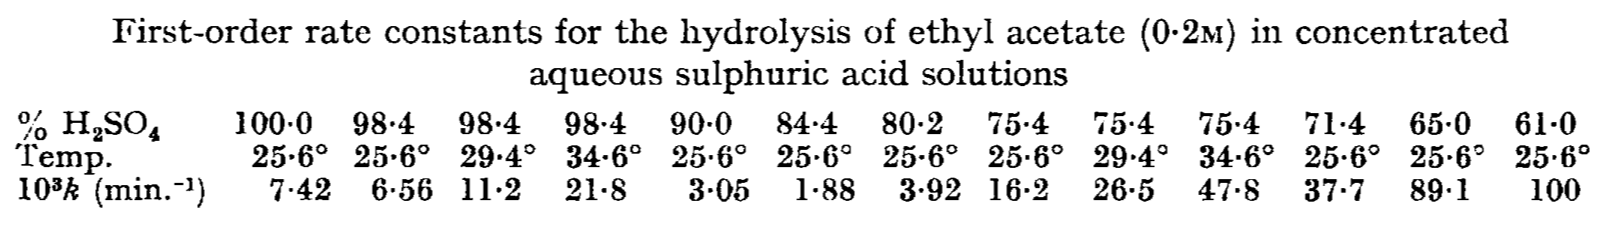
\includegraphics[scale=0.18]{images/jaquestable} 
  \caption[][0mm]{Data table~1 from Jaques, 1965\tss{\ref{ref:jaques}}  \\  $\longleftarrow$ \vspace{3mm}}

  \label{fig:jaques}
\end{figure}

Take note that Jaques reports rates at some temperatures other than \qty{25}{\degreeCelsius}. I will use only the data collected at \qty{25.6}{\degreeCelsius}.


\subsection{The Assembled EtOAc Data}

I took the data from Lane\tss{\ref{ref:lane}} \& Bell\tss{\ref{ref:bell}} and combined it with the data from Jaques\tss{\ref{ref:jaques}} to obtain the data set for the hydrolysis of ethyl acetate in a wide range of mixtures of sulphuric acid. I had to convert the rate units from $\text{s}^{-1}$ and $10^3\,\text{min}^{-1}$ to $10^2\,\text{min}^{-1}$ to match the data set for ester hydrolysis presented in table~1 of Yates.\tss{\ref{ref:ref1}} Table~\vref{tab:final} contains the assembled data set for rates of ethyl acetate hydrolysis at \qty{25}{\degreeCelsius}.

Figure~\vref{fig:yates_redone} shows a plot of this data for EtOAc along with the data for the alkyl esters. I observed that my own data set, that was assembled from the combined data set reported by Lane\tss{\ref{ref:lane}} and the stronger acid conditions reported by Jaques,\tss{\ref{ref:jaques}} contained more points than shown on the plot that was presented as Figure~1 in Yates\tss{\ref{ref:ref1}}. After close inspection of the image, I observe that Yates \& McClelland did not use the experimental data reported by Lane, but selected only the data that had been previously reported by Bell.\tss{\ref{ref:bell}}  Yates and McClelland had referenced data for EtOAc hydrolysis from Lane, but they only used data from Bell and Jaques. Although, to be fair, the experimental results from Lane were``in press'' when this paper was published, and the reference to that work was likely a late addition to the paper after the work had been done.

I will include the experimental data from Lane in the data sets as I re-analyze the data. The combined data set for ETOAc hydrolysis is collected in Table~\ref{tab:final}.

\begin{figure}[h!]
\vspace{0mm}
  \centering
  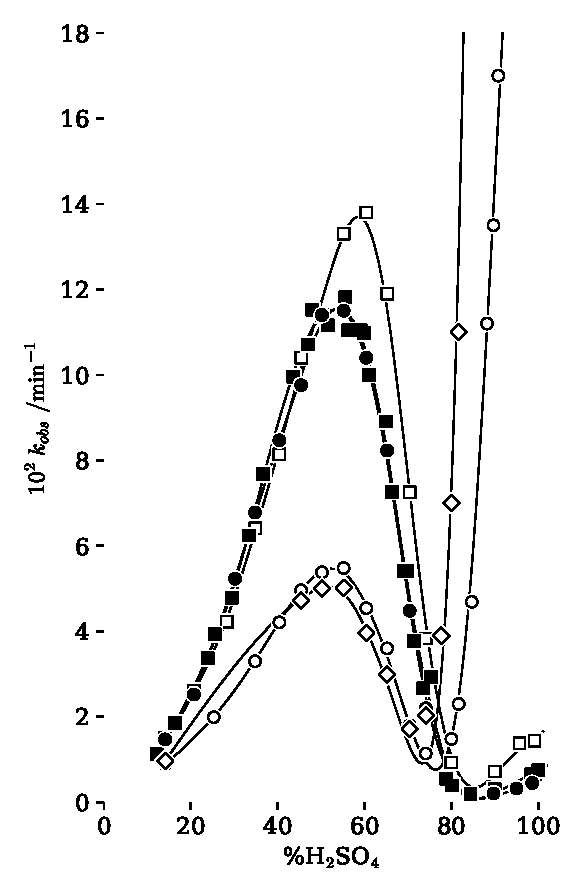
\includegraphics[scale=0.7]{images/plot5_combo} 
  \caption[][-0mm]{Plot of the assembled hydrolysis rate data for alkyl esters. Compare this to Figure~1 in Yates, 1967.\tss{\ref{ref:ref1}}.

\includegraphics[width=5pt]{images/symbols/OpenSquare} MeOAC, \\
 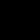
\includegraphics[width=5pt]{images/symbols/FilledSquare} ETOAc,
 
\includegraphics[width=5pt]{images/symbols/FilledCircle} nPrOAc,
 
\includegraphics[width=5pt]{images/symbols/OpenCircle} iPrOAc,\\
  
\includegraphics[width=5pt]{images/symbols/OpenDiamond} sec-BuOAc. The lines are smoothed interpolations and have no mathematical meaning.  \\  $\longleftarrow$\vspace{1mm}}

  \label{fig:yates_redone}
\end{figure}

\begin{margintable}[-60mm]
\caption{Collected data for rates of ethyl acetate hydrolysis in sulphuric acid mixtures at \qty{25}{\degreeCelsius}. The sources of the data are a) Lane\tss{\ref{ref:lane}} \& Bell\tss{\ref{ref:bell}}, b) Lane\tss{\ref{ref:lane}}, and c) Jaques.\tss{\ref{ref:jaques}}  \vspace{1mm} }

\centering
    \begin{tabular}{SSc}
%        \toprule
{\%\ce{H2SO4}}  & {$k_{obs}\ /10^{-2}\,\text{min}^{-1}$} & {source} \\
        \midrule
12.2  &      1.128  &   a  \\ 
16.4  &      1.854  &   a  \\ 
23.9  &      3.366  &   a  \\ 
25.5  &      3.93  &    a  \\ 
29.4  &      4.782  &   a  \\ 
33.43  &     6.24  &    a  \\ 
36.67  &     7.68  &    a  \\ 
43.56  &     9.96  &    a  \\ 
47.00  &    10.71  &    b  \\
48.00  &    11.52  &    a  \\ 
51.55  &    11.16  &    b  \\
55.6  &     11.82  &    b  \\
56.25  &    11.04  &    b  \\
59.18  &    11.04  &    b  \\
59.88  &    10.98  &    b  \\
61.0  &     10.0  &     c  \\  
65.0  &      8.91  &    c  \\  
66.32  &     7.26  &    b  \\
68.97  &     5.418  &   b  \\
69.88  &     5.418  &   b  \\
71.4  &      3.77  &    c  \\ 
73.55  &     2.664  &   b  \\
75.4  &      2.94   &   c  \\
78.8  &      0.551  &   b  \\
80.2  &      0.392  &   c  \\ 
84.4  &      0.188  &   c  \\ 
90.0  &      0.305  &   c  \\ 
98.4  &      0.656  &   c  \\ 
100.0  &     0.746  &   c  \\ 
%        \bottomrule
    \end{tabular} 
    \label{tab:final}
\end{margintable}


\section{The Final Data Set}

For the record, I will present the data set that will be used in the analysis as we explore this work. The data set obtained from the literature references for EtOAc hydrolysis are presented in Table~\vref{tab:final} and data for the other esters as reported in Yates \& McClelland, 1967\tss{\ref{ref:ref1}} are reproduced in Tables~\ref{tab:all1}, \ref{tab:all2}, \ref{tab:all3} and \ref{tab:all4} on the following pages. 


\begin{table}
    \caption{Collected data for rates of primary alkyl ester hydrolysis in sulphuric acid mixtures: methyl acetate and n-propyl acetate. This data if from table~1 of Yates\tss{\ref{ref:ref1}} and includes the three data points for MeOAc hydrolysis that were observed in the plot of Figure~1 in Yates, but were absent in the published data. Temp = \qty{25}{\degreeCelsius}\\ $\longleftarrow$\\ \vspace{10mm}
\textsc{Note}: the adjusted values for the digitized data points for MeOAc would have set the highest concentrations at 89.65, 95.32 and 98.76 \%\ce{H2SO4}. It is very likely that the smilar concentration values reported for nPrOAc are, in fact, the concentrations used. I used the concentrations values of 89.7, 95.0 and 98.6 \%\ce{H2SO4} that matched the nPrOAc data set.}
\centering
    \begin{tabular}{lSS}
%        \toprule

{Ester} & {\%\ce{H2SO4}} &  {$10^{-2}\,k_{obs}\;/\text{min}^{-1}$}    \\ 
        \midrule     
{\ce{MeOAc}} & 14.1&     1.50    \\ 
 &       20.7&          2.61    \\ 
 &       28.3&          4.22    \\ 
 &       34.8&          6.41    \\ 
 &       40.4&          8.14    \\ 
 &       45.4&         10.4    \\ 
 &       50.2&         11.4    \\ 
 &       55.2&         13.3    \\ 
 &       60.4&         13.8    \\ 
 &       65.2&         11.9    \\ 
 &       70.4&          7.25    \\ 
 &       74.1&          3.83    \\ 
 &       80.0&          0.931    \\ 
 &       89.7&         0.72       \\ 
 &       95.0&         1.38       \\ 
 &       98.6&         1.44       \\ 
 
 
 
        \midrule     
{\ce{nPrOAc}}&14.1&    1.47    \\ 
 &      20.7&          2.52    \\ 
 &      30.2&          5.23    \\ 
 &      34.8&          6.78    \\ 
 &      40.4&          8.47    \\ 
 &      45.4&          9.76    \\ 
 &      50.2&         11.4    \\ 
 &      55.2&         11.5    \\ 
 &      60.4&         10.4    \\ 
 &      65.2&          8.23    \\ 
 &      70.4&          4.48    \\ 
 &      74.1&          2.20    \\ 
 &      89.7&          0.205    \\ 
 &      95.0&          0.323    \\ 
 &      98.6&          0.450    \\ 
    \label{tab:all1}

    \end{tabular} 

\end{table}




\begin{table}
    \caption{Collected data for rates of secondary alkyl ester hydrolysis in sulphuric acid mixtures: isopropyl acetate and sec-butyl acetate.  Temp = \qty{25}{\degreeCelsius}\\ $\longleftarrow$}

\centering
    \begin{tabular}{lSS}
%        \toprule

{Ester} & {\%\ce{H2SO4}} &  {$10^{-2}\,k_{obs}\;/\text{min}^{-1}$}    \\ 
\midrule
{\ce{iPrOAc}}& 14.1&   0.890    \\ 
 &      25.3&          1.99    \\ 
 &      34.8&          3.30    \\ 
 &      40.4&          4.21    \\ 
 &      45.4&          4.96    \\ 
 &      50.2&          5.38    \\ 
 &      55.2&          5.48    \\ 
 &      60.4&          4.54    \\ 
 &      65.2&          3.60    \\ 
 &      70.4&          1.80    \\ 
 &      74.1&          1.14    \\ 
 &      80.0&          1.48    \\ 
 &      81.7&          2.30    \\ 
 &      84.7&          4.69    \\ 
 &      88.2&         11.2    \\ 
 &      89.7&         13.5    \\ 
 &      90.8&         17.0    \\ 
 \midrule
{{sec-BuOAc}}& 14.1& 0.964    \\ 
 &    45.4&          4.72    \\ 
 &    50.2&          5.00    \\ 
 &    55.2&          5.02    \\ 
 &    60.4&          3.96    \\ 
 &    65.2&          2.99    \\ 
 &    70.4&          1.71    \\ 
 &    74.1&          2.03    \\ 
 &    77.7&          3.90    \\ 
 &    80.0&          7.00    \\ 
 &    81.7&         11.00    \\ 
 &    84.7&         23.6    \\ 
 &    88.2&         63.2    \\ 
 
 
     \label{tab:all2}

    \end{tabular} 

\end{table}

\begin{table}
    \caption{Collected data for rates of benzyl acetate hydrolysis in sulphuric acid mixtures.  Temp = \qty{25}{\degreeCelsius}\\ $\longleftarrow$}

\centering
    \begin{tabular}{lSS}
%        \toprule

{Ester} & {\%\ce{H2SO4}} &  {$10^{-2}\,k_{obs}\;/\text{min}^{-1}$}    \\ 
        \midrule   
{\ce{BnOAc}}& 10.1&     0.74    \\ 
 &       25.3&          2.52    \\ 
 &       30.2&          4.04    \\ 
 &       34.8&          4.61    \\ 
 &       40.4&          6.08    \\ 
 &       45.4&          7.13    \\ 
 &       50.2&          9.81    \\ 
 &       52.8&          9.30    \\ 
 &       55.2&          9.91    \\ 
 &       60.4&          8.52    \\ 
 &       62.5&          9.24    \\ 
 &       65.2&         10.1    \\ 
 &       66.8&         13.7    \\ 
 &       67.3&         15.7    \\ 
 &       69.0&         22.3    \\ 
 
 
  
     \label{tab:all3}

    \end{tabular} 

\end{table}

 
 
\begin{table}
    \caption{Collected data for rates of substituted phenyl ester hydrolysis in sulphuric acid mixtures: phenyl acetate, p-chlorophenyl acetate and p-nitrophenyl acetate.  Temp = \qty{25}{\degreeCelsius}\\ $\longleftarrow$}

\centering
    \begin{tabular}{lSS}
%        \toprule

{Ester} & {\%\ce{H2SO4}} &  {$10^{-2}\,k_{obs}\;/\text{min}^{-1}$}    \\ 
\midrule
{\ce{PhOAc}}&  15.1&    1.08    \\ 
 &       20.1&          1.62    \\ 
 &       25.3&          2.38    \\ 
 &       30.2&          3.30    \\ 
 &       34.8&          4.34    \\ 
 &       40.4&          6.20    \\ 
 &       45.4&          8.36    \\ 
 &       50.2&         10.9    \\ 
 &       55.2&         14.5    \\ 
 &       60.4&         19.2    \\ 
 &       65.2&         22.6    \\ 
 &       70.4&         27.2    \\ 
 &       74.1&         29.3    \\ 
\midrule
{\ce{p-ClPhOAc}}& 15.1&  0.922    \\ 
 &   34.8&          4.25    \\ 
 &   45.4&          7.90    \\ 
 &   55.2&         13.4    \\ 
 &   65.2&         22.7    \\ 
 &   70.4&         27.3    \\ 
 &   74.1&         38.2    \\ 
\midrule
{\ce{p-NO2PhOAc}}& 15.1& 0.751    \\ 
 &  20.1&          1.12    \\ 
 &  25.3&          1.52    \\ 
 &  30.2&          2.36    \\ 
 &  34.8&          3.09    \\ 
 &  40.4&          4.27    \\ 
 &  45.4&          5.71    \\ 
 &  50.2&          7.81    \\ 
 &  55.2&         10.8    \\ 
 &  60.4&         15.2    \\ 
 &  65.2&         21.3    \\ 
 &  70.4&         36.1    \\ 
 &  74.1&         70.5    \\ 
 &  75.3&         93.3    \\ 
 &  77.7&        161    \\ 
 &  78.5&        158    \\ 
 &  80.0&        222     \\

    \label{tab:all4}

    \end{tabular} 

\end{table}

\end{document}
